\subsubsection{01.12.14}

\begin{enumerate}
	\item Время начала и окончания собрания:
	15:30 - 19:00
	\item Цели собрания:
	\begin{enumerate}
	  \item Переместить механизм опрокидывания ковша на самый верх последней мебельной рейки.
	  
	  \item Установить П-образное ребро жесткости.
	  
	  \item Начать разработку концепции ковша.
	  
    \end{enumerate}
	\item Проделанная работа:
	\begin{enumerate}
	  \item Механизм опрокидывания ковша был перемещен на верх последней мебельной рейки.
	  
	  \begin{figure}[H]
	  	\begin{minipage}[h]{0.2\linewidth}
	  		\center  
	  	\end{minipage}
	  	\begin{minipage}[h]{0.6\linewidth}
	  		\center{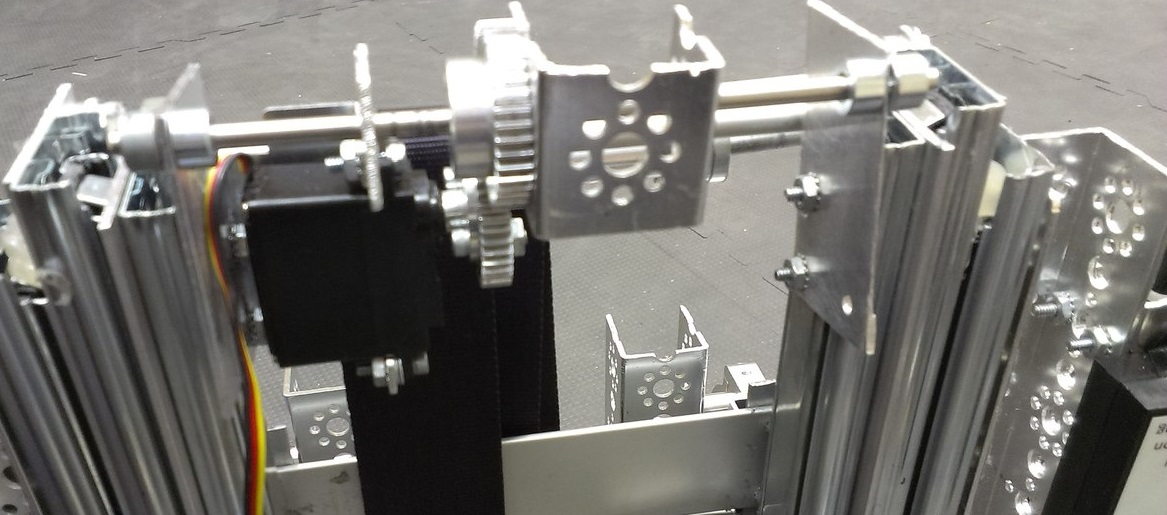
\includegraphics[scale=0.2]{days/01.12.14/images/01}}
	  		\caption{Механизм опрокидывания ковша}
	  	\end{minipage}
	  \end{figure}
	  
	  \item П-образное ребро жесткости не было установлено.
	  
	  \item Было решено создать ковш таким образом: снизу идет поддон высотой 7 см, к передней стенке которого прикреплен пандус (трамплин, по которому захват будет проталкивать мячи в ковш). Затем идет часть, открытая спереди, чтобы мячи могли попадать внутрь ковша. Еще выше ковш начинает равномерно сужаться и на самом верху имеет выходное отверстие размерами чуть больше размеров большого мяча (7 см). Равномерное сужение не позволит мячам застревать внутри ковша. За ковшом идет наклонный желоб, неподвижно закрепленный на верхней паре мебельных реек так, что мячи, выпадающие из опрокинутого ковша, попадают прямо в него. Желоб заканчивается откидной деталью с отверстием в дне, расположенном так, чтобы мячи падали из него строго вертикально вниз - это повысит точность захватывания. Откидная часть должна быть сделана так, чтобы в сложенном состоянии она входила в габариты, а в разложенном - ее отверстие располагалось прямо над подвижной корзиной, захваченной роботом.
	  
	  \begin{figure}[H]
	  	\begin{minipage}[h]{0.2\linewidth}
	  		\center  
	  	\end{minipage}
	  	\begin{minipage}[h]{0.6\linewidth}
	  		\center{
\includegraphics[scale=0.2]{days/01.12.14/images/02}}
	  		\caption{Концепция ковша}
	  	\end{minipage}
	  \end{figure}
	  
    \end{enumerate}
    
	\item Итоги собрания: 
	\begin{enumerate}
	  \item Механизм опрокидывания ковша перемещен на верх мебельной рейки.
	  
	  \item Ребро жесткости не установлено.
	  
    \end{enumerate}
    
	\item Задачи для последующих собраний:
	\begin{enumerate}
	  \item Установить П-образное ребро жесткости.
	  
	  \item Начать реализацию проекта нового ковша.
	  
    \end{enumerate}     
\end{enumerate}
\fillpage